\textit{In this chapter, detailed information of the design and implementation process of the WSN control system is provided based on what was recorded during the literature review. Furthermore, detailed theory of the two control strategies is discussed.}

\section{WSN Simulation Environment}
 In order to make unbiased comparisons between the two controllers' performances, all tests had to be executed in an identical simulation environment. Based on the grounds that the WSN simulation environment needed to mainly be energy-oriented to answer the research questions, there were not any ideal pre-built simulators. Instead it was decided to develop and build a WSN environment which focused on the energy consumption of the nodes in the WSN. The WSN environment was developed using the equations governing the energy \& data aggregation as stated in Subsection \ref{subsec:sinkDataFlow} and consisted of three classes together with a script for visualizing the environment. See Figure \ref{fig:WSNUML} for a UML representation of the WSN simulation environment. 

\begin{figure}
    \centering
    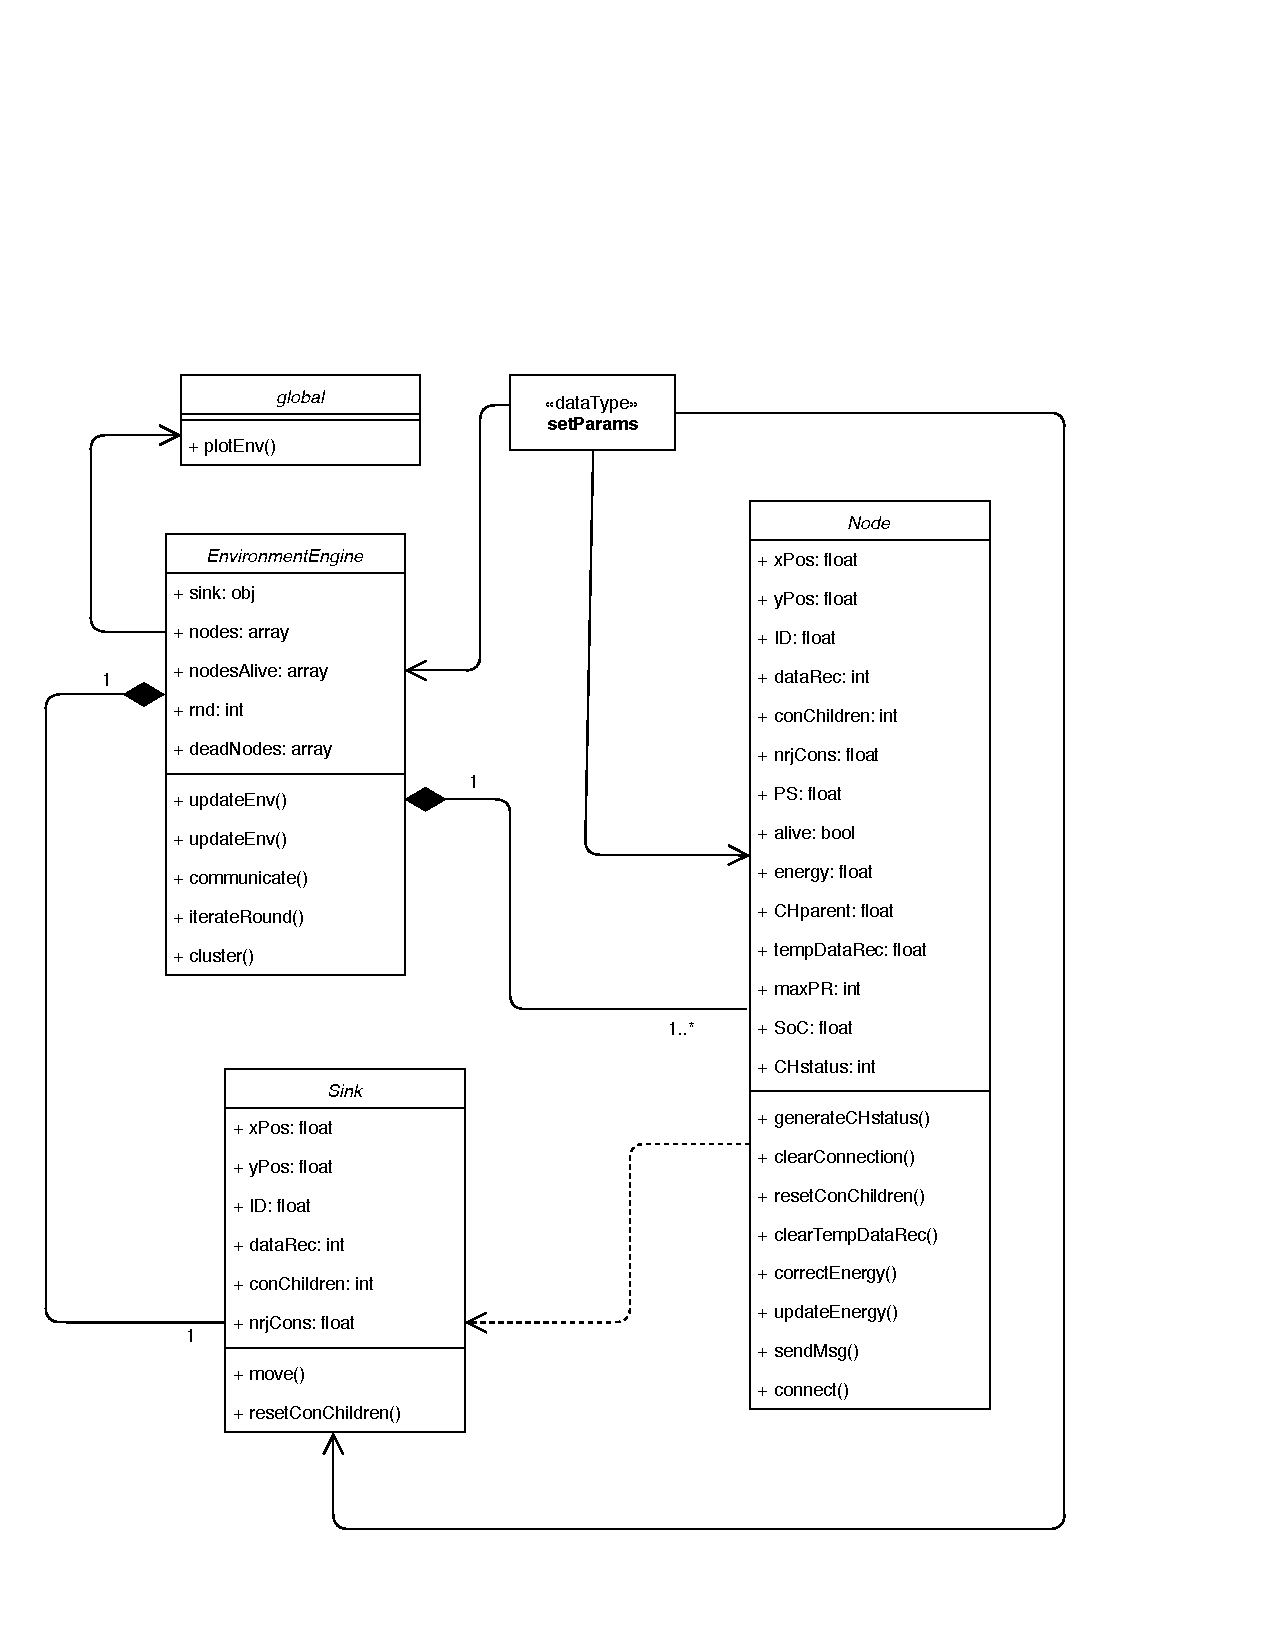
\includegraphics[scale=.7]{Images/WSNUML.pdf}
    \caption{UML of WSN simulation environment}
    \label{fig:WSNUML}
\end{figure}

 \subsection{Simulation Environment Architecture}
 \subsubsection{Sink}
 The mobile sink was represented as an object with the \verb!Sink! class. By using the size of the WSN environment the \verb!Sink! object was always placed in the middle when it was initiated. The most pivotal method of this class is named \verb!move()! which enabled movement of the sink in any direction.     

 \subsubsection{Node}
 The \verb!Node! class was used to represent one node in the simulation environment. When a node was created it required a node ID number, $x$- \& $y$-position and an initial energy level as input. After an instance of the node was created, methods such as \verb!generateCHstatus()!, \verb!connect()!, \verb!sendMsg()! and \verb!updateEnergy()! were utilized to decide whether the node's CH status, connect to the sink or another node, send data messages and update the node's energy after sending and/or receiving data respectively. 

 \subsubsection{EnvironmentEngine}
 \noindent The \verb!EnvironmentEngine! class had the responsibility of interlinking the different modules of the WSN environment. By holding onto one \verb!Sink! object and numerous \verb!Node! objects the \verb!EnvironmentEngine! class linked together the modules with its methods. The \verb!cluster()! method elected CHs, \verb!updateEnv()! method moved the sink \& changed the PR of the nodes, \verb!communicate()! method sent the messages between nodes \& nodes/sink and the \verb!iterateRound()! method was used to reset some attributes before the start of a new round.

\subsubsection{Main script}
To visualize the WSN and its performance, a function based on the \verb!Matplotlib! library was implemented. This function plotted the sink and the nodes in a 2D grid as well as which of the nodes were CHs. The performance of the controllers were depicted in real time as plots of energy consumed, amount of dead nodes and amount of data packets sent as a function of the current round. \newline

\noindent To simulate the behaviour of the system, the interaction of the classes were put in a loop designed to break if the environment engine detected 0 alive nodes. During each loop, three actions were repeated until network failure, see Figure \ref{fig:mainscriptflowchart}.
\begin{figure}
    \centering
    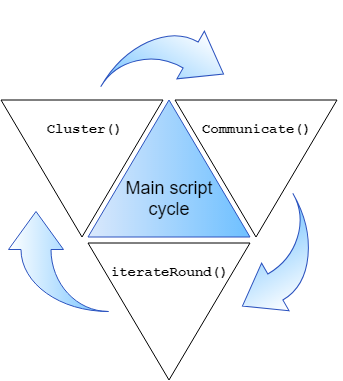
\includegraphics[scale = 0.45]{Images/mainscriptflowchart.png}
    \caption{Main script action sequence for each loop until network failure.}
    \label{fig:mainscriptflowchart}
\end{figure}
In order to control the network, each transmission round was split into a minor loop of a set number of time segments. During each time segment, each CH was allowed to execute \verb!sendMsg()! with a regulated amount of packages. \newline


\subsubsection{Distributed- Versus Random-Mode}
Two different settings were implemented in order to be able to choose whether the nodes should all begin with the same amount of energy or if they should begin with a randomized amount of energy. \verb!distr! signaled that each node would start with the same energy, while \verb!rand! meant that each node would start with $E=rand(1)\cdot Max\:energy$. The purpose of the random mode was to simulate a real world application where energy consumption, and generation, could be stochastic or favoured in certain areas.

\subsubsection{Environment Parameters}
\noindent Table \ref{tb:Envdesign} depicts the parameter values that were used during simulations.  

\begin{table}[h!]
    \centering
    \caption{Environment parameter choices}
    \label{tb:Envdesign}
    \begin{tabular}{ 
        l % left aligned column
        l % left aligned column
        *{3}{S[table-format=4.0]} % three columns with numeric data       
    }
        \toprule
        \textbf{Parameter} & \textbf{Value}  \\ 
        \midrule
        $x \: size$ & $100 \: m$ \\ \\[-1em]
        $y \: size$ & $100 \: m$ \\ \\[-1em]
        $Max \: energy$ & $0.05 \: J$ \\ \\[-1em]
        $E_{elec}$ & $ 50 \cdot 10^{-9} \: \frac{J}{bit}$ \\ \\[-1em]
        $E_{Tx}$ & $ 50 \cdot 10^{-9} \: \frac{J}{bit}$ \\ \\[-1em]
        $E_{Rx}$ & $ 50 \cdot 10^{-9} \: \frac{J}{bit}$ \\ \\[-1em]
        $E_{amp}$ & $ 10^{-10} \: \frac{J}{bit \cdot m^{2}}$ \\ \\ [-1em]
        $E_{DA}$ & $ 50 \cdot 10^{-9} \: \frac{J}{bit}$ \\ \\[-1em]
        $Time\:segments$ & $10$\\ \\[-1em]
        $Mode$ & $'distr'\: or \: 'rand'$\\ \\[-1em]
        \bottomrule
    \end{tabular}
\end{table}



\section{BLEACH}
The broadening of the LEACH protocol equation, now called BLEACH (Broadened LEACH), was to have the term $SoC$ included. Here, $SoC\in[0,1]$ was defined as the percentual amount of energy stored in the node.
\begin{equation}
    SoC = \frac{E_{current\:battery}}{E_{max\:battery}}
\end{equation}
Several requirements and soft goals were created for the BLEACH equation.
\begin{enumerate}
    \item The equation shall be able to produce CHs at any round as long as there are nodes are alive which have elected during the current episode
    \item The influence of the $SoC$- and round-dependency shall be dynamic and adjustable
    \item The equation shall only involve variables and parameters available to the individual node
    \item It would be beneficial if the amount of CHs relative to the total number of nodes is similar for each round
    \item It would be beneficial for the equation to function as regular LEACH when there is little to no difference in $SoC$
\end{enumerate}
\noindent If the established requirements for the expression was deemed as satisfied, the development process was to move on towards testing for analyzing of results, see Chapter \ref{ch:Methodology}.

\subsection{BLEACH Expression Design}
A direct coupling of the $SoC$ to the LEACH expression $T_{LEACH}$, see Equation \ref{leacheq}, would result in lowering the overall $T$-value among the nodes; as soon as energy runs low in the network, little to no CH roles would be produced. In response to this, the BLEACH expression was divided into two functions $S(n, SoC)$ and $R(n)$, see Equation \ref{SandR}. One term was to be dependant on the $SoC$, and the other only dependant on the current round. 
\begin{equation}
    \label{SandR}
    T_{BLEACH}(rnd, SoC) = (1-f)\cdot S + f\cdot R
\end{equation}
The weight factor $f$ was introduced in order to regulate the total value of $T_{BLEACH}$. To retain the behaviour of the former equation, both
$S$ and $R$ were based on the original expression. \newline
The following definitions were formed
\begin{align}
    \label{SandRexpanded}
    S &= h_s\frac{P}{1-P(rnd\,mod\frac{1}{P})}SoC = h_s\cdot T_{LEACH} \cdot Soc\\
    R &= h_r\cdot C \cdot \frac{P}{1-P(r\,mod\frac{1}{P})} = h_r \cdot C \cdot T_{LEACH}\\
    C &= \frac{1}{1-(1-f)\big(\frac{P}{1-P(r\,mod\frac{1}{P})}\big)} = \frac{1}{1-(1-f)T_{LEACH}}
\end{align}
\noindent A mechanism was required to ensure that CHs were chosen with a similar distribution despite energy being low on all nodes. This was the purpose of the additional parameter $h_s$ in $S$ and the additional factor $C$ in $R$. 
$C$ works by gradually nullifying $f$ towards the end of the cycle. For example, if $h_r = 1$ and $r = \frac{1}{P}-1$ (the last round index of the cycle), we have that
\begin{align}
    C = \frac{1}{f} \\
    f\cdot R = f\cdot C \cdot \frac{P}{1-P(r\,mod\frac{1}{P})} = T_{LEACH}
\end{align}

thus making sure that $T\geq1$ is guaranteed for the remaining nodes at the last round. However, a value of $R\geq1$ is not desired for all nodes at the final round; if each node was guaranteed to become a CH during each cycle, the $SoC$-prioritization would serve no purpose. Therefore, the factor $h_r$ was introduced to control the impact of $R$ so as to keep $T_{BLEACH}(\frac{1}{P})$ below 1 for nodes with $SoC$ below a certain value.\newline

\noindent The parameter $h_s$ decides in which range $S$ can vary. If $h_s\not> 1$, then $T_{BLEACH}$ would assume lesser values than $T_{LEACH}$ at each round where $f\cdot C \leq f$ regardless of $SoC$, as seen in Equation \ref{h_sproof}.\newline
For $h_s,h_r = 1$
\begin{align}
    \label{h_sproof}
    T_{BLEACH} = f\cdot S + (1-f)\cdot R = &f\cdot T_{LEACH}\cdot SoC + (1-f)\cdot C \cdot T_{LEACH} \\
    for\;&SoC\in[0,1], \nonumber \\
    &\Downarrow \nonumber \\
    T_{BLEACH} = T_{LEACH}(1&+f(SoC-1))\leq T_{LEACH} \nonumber
\end{align}

\noindent The expression modifications were continuously observed in MATLAB to evaluate their behaviour with respect to the previously mentioned requirements. The observations where made at different stages of a cycle at different levels of $SoC$, see Figure \ref{fig:B_LEACHplots}. 


\begin{figure}
    \centering
    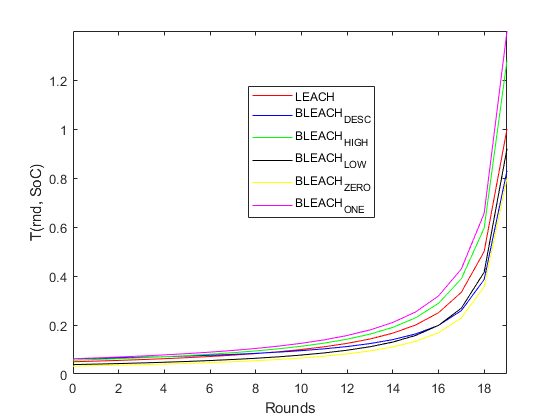
\includegraphics[scale=0.9]{Images/B_LEACHallPlots.png}
    \caption{Value of $T$ over one cycle for $P=0.05$, $f=0.8$, $h_s=3$ and $h_r = 0.8$ for LEACH and BLEACH with varying $SoC$. $BLEACH_{HIGH}$ represents a constantly high value of $SoC = 0.8$, $BLEACH_{LOW} \Rightarrow SoC = 0.2$, $BLEACH_{ONE} \Rightarrow SoC=1$, $BLEACH_{ZERO} \Rightarrow SoC=0$, and $BLEACH_{DESC}$ plots a decreasing value of $SoC \in [1 0]$. $T_{BLEACH}$ exhibits a behaviour similar to $T_{LEACH}$. However, the values are distributed on both sides of the original depending on the node's $SoC$.}
    \label{fig:B_LEACHplots}
\end{figure}

\subsubsection{Simplified BLEACH}
As an alternative to the more complex former expression, an additional approach was offered.
As previously discussed, there was reason to believe that a $T$-value varying between values close to $T_{LEACH}$ depending on $SoC$ was to be beneficial. This solution works by implementing a look-up table of size $100\times L_{cycle}$, where $L_{cycle}$ is the amount of rounds in a cycle. The table is filled with scaled versions of $T_{LEACH}$ such that

\begin{align}
\hspace{-1.25cm}
\tiny
    \begin{bmatrix}
        (1-spread)\cdot T_{LEACH, n=1} & (1-spread)\cdot T_{LEACH, n=2} &\hdots& (1-spread)\cdot T_{LEACH, n=L_{cycle}} \\
        (1-spread+step)\cdot T_{LEACH, n=1} & (1-spread+step)\cdot T_{LEACH, n=2} &\hdots& (1-spread+step)\cdot T_{LEACH, n=L_{cycle}}\\
        (1-spread+2\cdot step)\cdot T_{LEACH, n=1} & (1-spread + 2\cdot step)\cdot T_{LEACH, n=2} &\hdots& (1-spread +2\cdot step)\cdot T_{LEACH, n=L_{cycle}}\\
        \vdots & \vdots & \ddots & \vdots \\
        (1+spread)\cdot T_{LEACH, n=1} & (1+spread)\cdot T_{LEACH, n=2} &\hdots& (1+spread)\cdot T_{LEACH, n=L_{cycle}}
    \end{bmatrix} 
\end{align}
where $step = \: 2 \frac{spread}{100}$ and $spread$ is the range of which the $T$-value is able to stray from the standard value of $T_{LEACH}$. The interval $[spread, spread+step, \hdots, spread+99\cdot step]$ is divided into 100 elements where each element corresponds to a scaling of $T_{LEACH}$, which is seen as a row in the table. In turn, each row corresponds to a specific value of $SoC$. For example, $spread=0.3$ and $SoC = 0.80$ would correspond to row $\# \: 80$ in the table which results in $(1-0.3+79\cdot step)\cdot T_{LEACH} = 1.174\cdot T_{LEACH}$.
The resulting spectrum of possible $T$-values can be seen in Figure \ref{fig:oBLEACH}.
\begin{figure}
    \centering
    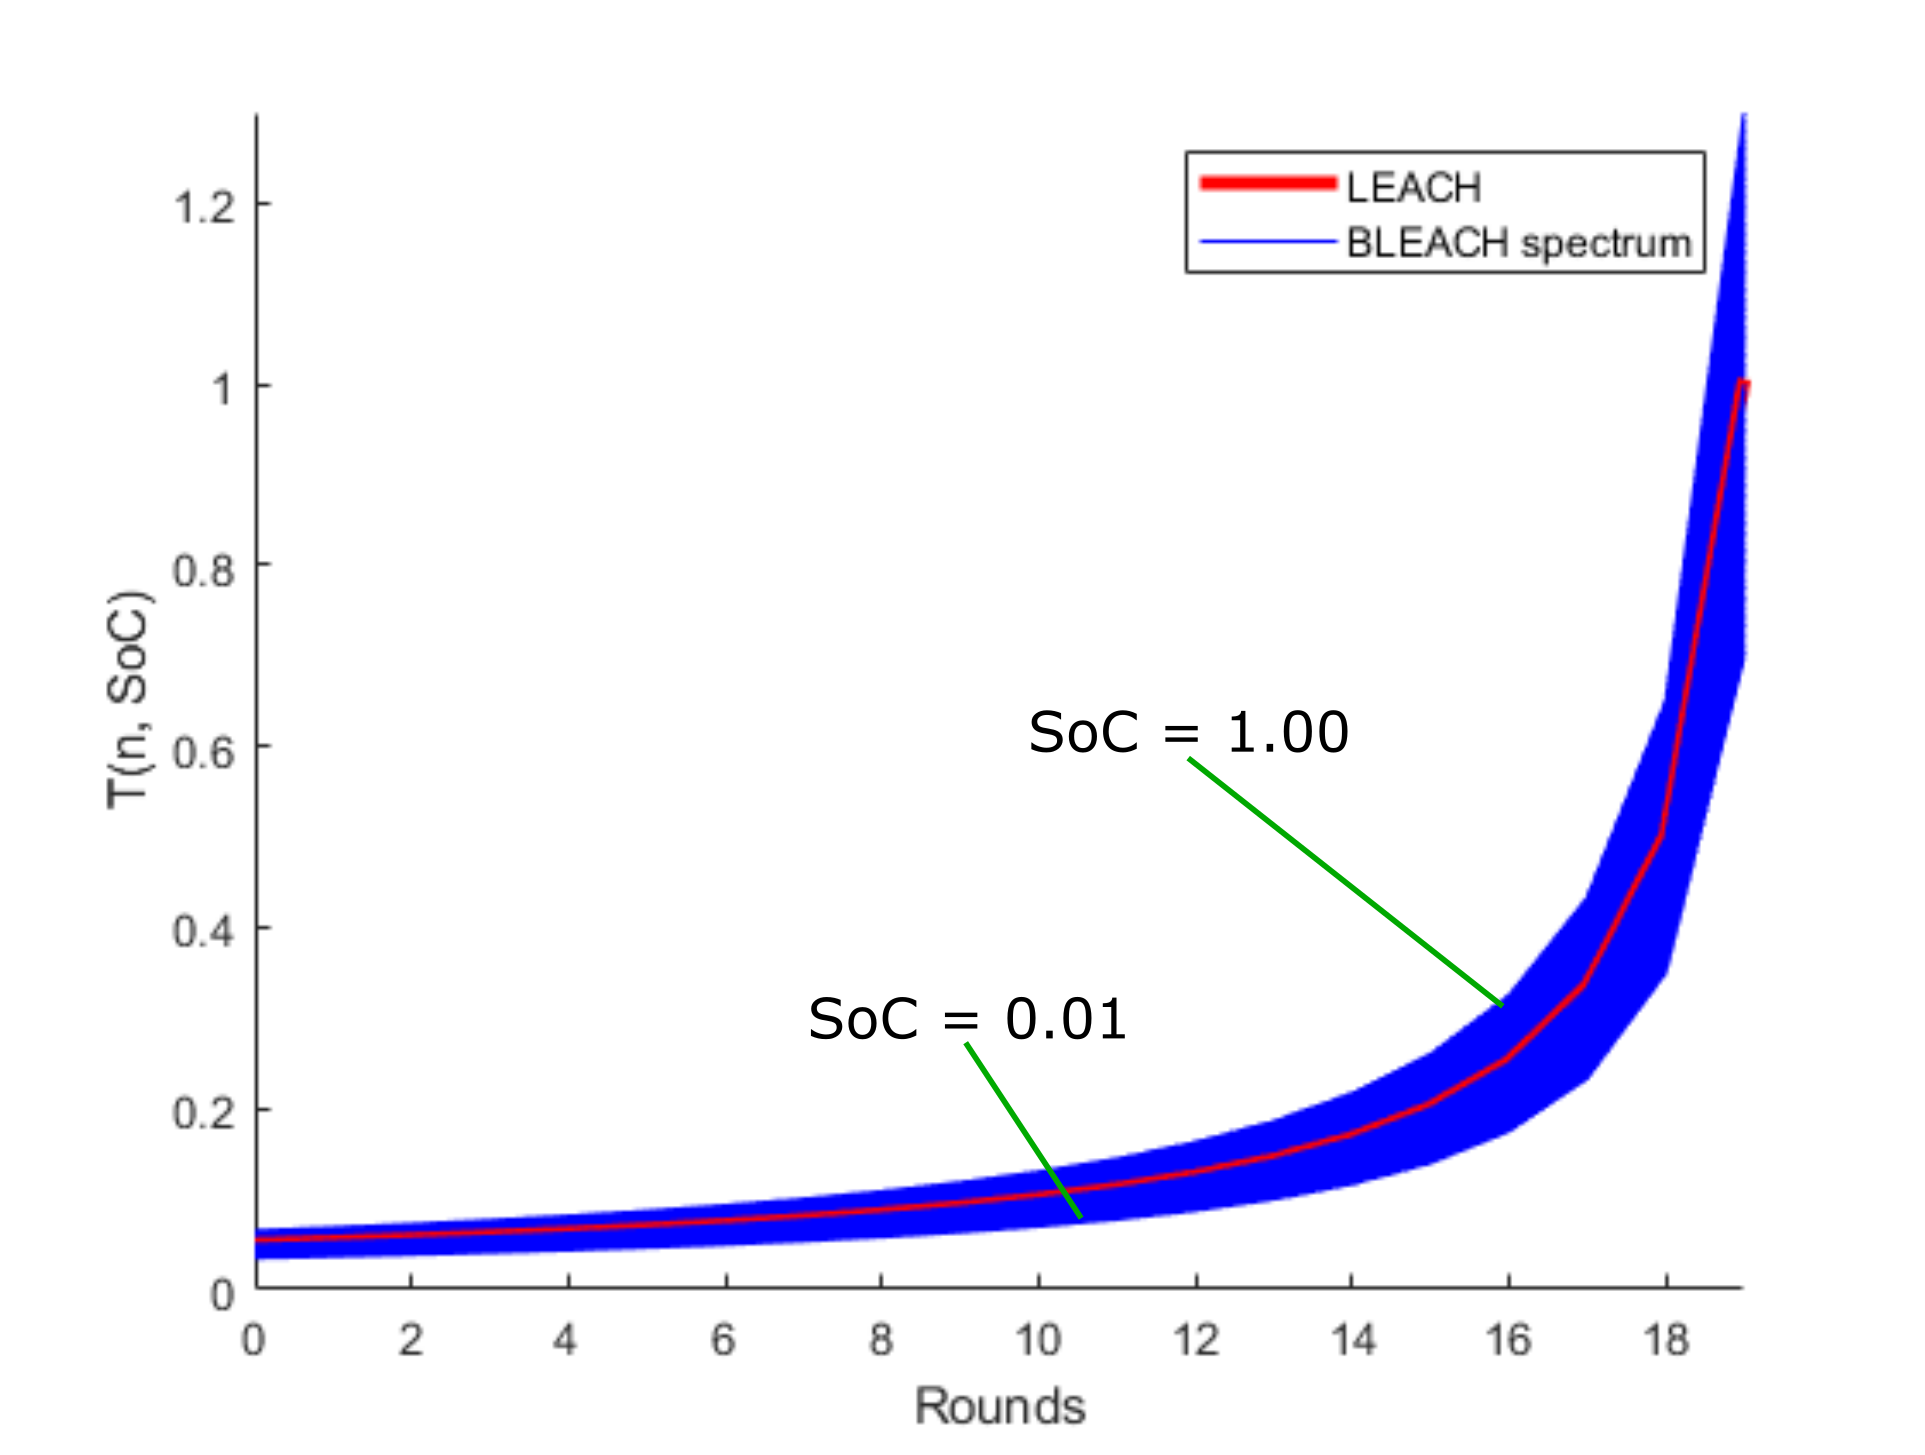
\includegraphics[scale=0.3]{Images/oBLEACH.png}
    \caption{Solution space for all possible $T$-values over a cycle for the simplified BLEACH-method. As demonstrated, $SoC\geq 0.5$ results in $T\geq T_{LEACH}$.}
    \label{fig:oBLEACH}
\end{figure}


\section{MPC Design}
Due to the advantages discussed in Chapter \ref{ch:LitReview}, NMPC was chosen as the model-based control strategy for the project. The proposed architecture of the controller-environment interaction can be seen in Figure \ref{fig:NMPCarchi}. Since the controller was to be implemented in a simulation environment devoid of any control disturbances or measurement noise, the state estimator part (as presented in \cite{findeisen2002introduction}) was not included.
\begin{figure}
    \centering
    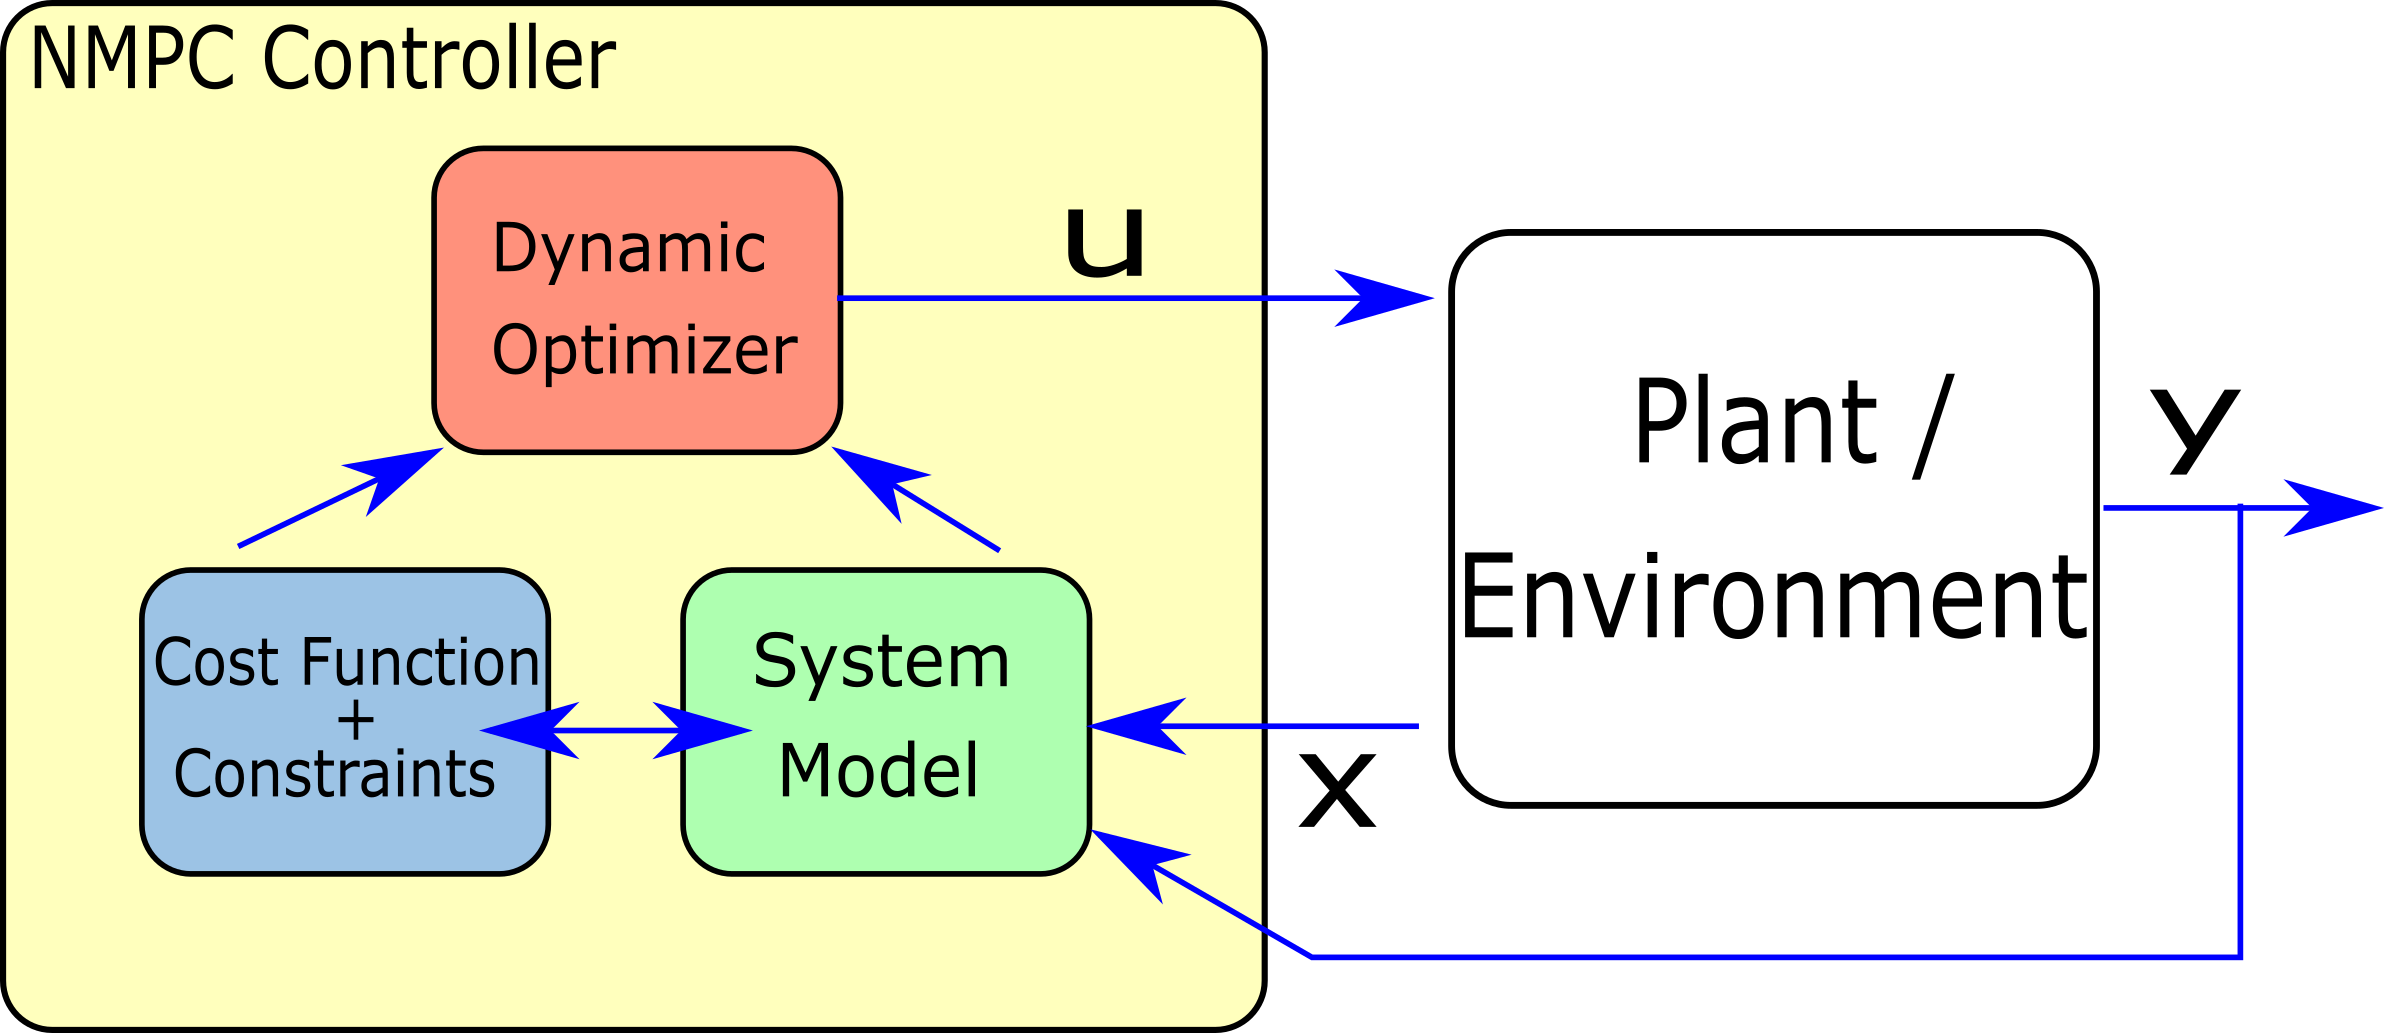
\includegraphics[scale=0.2]{Images/NMPCcontr.png}
    \caption{Basic NMPC control loop.}
    \label{fig:NMPCarchi}
\end{figure}

\noindent The complete optimal control problem was formulated with a mathematical model of the system. A corresponding MPC architecture with receding horizon was then designed and implemented with a chosen optimization tool. GEKKO was chosen over CasADi for this implementation due to its previously discussed benefits.\newline

\noindent The problem was to be solved by optimizing for a control sequence that minimizes a stated objective function $J$ depending on the two economic goals. Namely, the energy consumed and packets received by the sink. Energy consumed increases the cost while data received by the sink decreases it.
The state vectors \textbf{x}, \textbf{u} and \textbf{d}, representing states, control inputs, and disturbance, respectively are expressed in vector form as
\begin{align}
\label{x_k}
    \textbf{x} = [x_{sink}, y_{sink}, x_{1,\hdots,N}, y_{1,\hdots,N}, CHS_{1,\hdots,N}, PS_{1,\hdots,N}, EC_{1,\hdots,N}]^{T} \qquad x \in  \mathbb{R}^{5N+2}\\
    \textbf{u} = [\Delta x_{sink}, \Delta y_{sink}, PA_{1,\hdots,N}]^{T} \qquad u \in  \mathbb{R}^{N+2}\\
    \textbf{d} = [E_{gen,1\hdots,N}]^{T} \qquad d \in  \mathbb{R}^{N}
\end{align}

\noindent $N$ is the number of nodes and $(\Delta x_{sink}, \Delta y_{sink})$ is the change in position of the sink. The position of node $i,\:[1,...,N]$ nodes is assumed to be static. $PS_i$ is the amount of packets sent, $PA_i$ is a control input deciding how many packets to send each control step depending on the distance $d_i$ from each node $i$ to the sink, $EC_i$ is energy consumed, and $E_{gen}$ is a node's generated energy modeled as a disturbance. Cluster head status $CHS_i \in [0,1]$ is an indicator of whether the node has been chosen to be a cluster head or not which would decide if control is to be executed with regards to that node. \newline

\noindent As mentioned in Section \ref{nonlinMPC}, with an increasing number of nodes the dimension of the state space increases at a problematic rate. For example, 100 nodes with 5 controlled inputs, as well as a sink a sink with 2, over a horizon $K=10$ (the previously specified number of time segments per transmission round) would result in near $1.3\cdot10^{11}$ computations per control step.
To circumvent this, a strategy involving breaking down the optimization problem for the entire state space into minor optimization problems was deployed.\newline

\noindent As shown in Figure \ref{fig:splitctrl}, one lower layer optimization problem is stated for each node, with $x_{node},\:u_{node}$, as well as one upper layer for the sink with state vector, $x_{sink}, \: u_{sink}$. With this architecture, the $\mathcal{O}$-notation based on the previous example could be reduced to a worst case at approximately $100\cdot(5\cdot10)^{3}<1.3\cdot10^{7}$ computations per control step. 
\begin{figure}
    \centering
    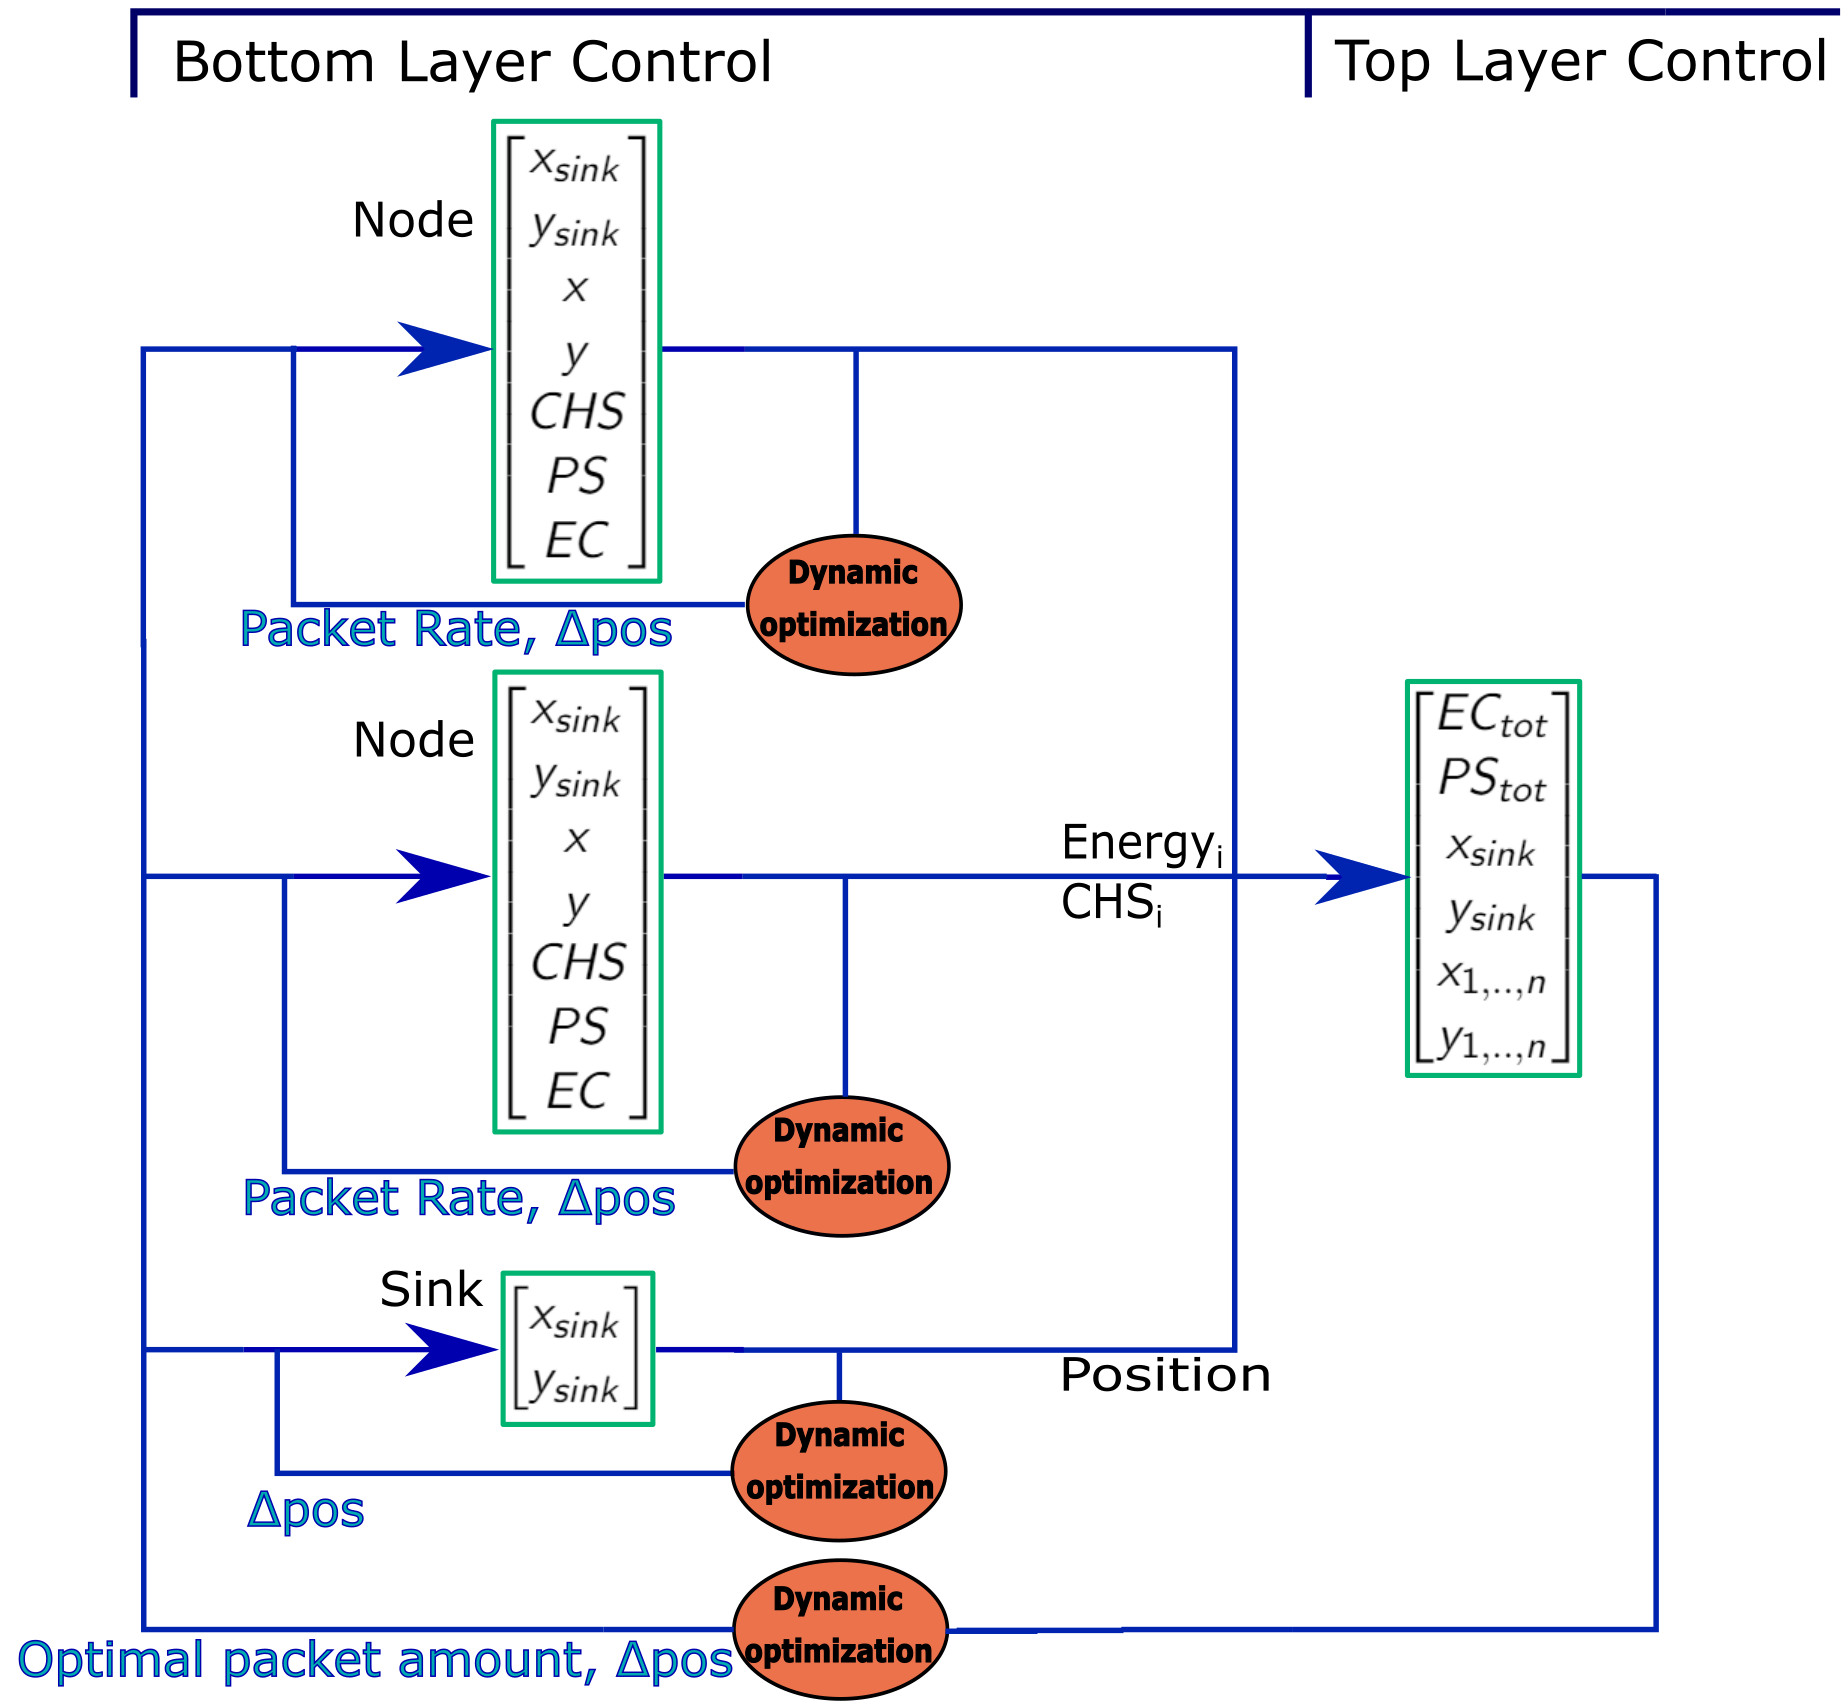
\includegraphics[scale = 0.4]{Images/splitcontrol.png}
    \caption{Architecture for the multi-layer control cooperation.}
    \label{fig:splitctrl}
\end{figure}
\subsection{Upper Layer Control}
\noindent The upper layer control (ULC) aims to solve for an optimal position of the sink as well as an optimal total amount of packets to be sent by each active CH during a transmission round. Since the setup of CHs changes completely as well as in a stochastic manner between every transmission round, planning for control signals beyond the current transmission round was not striven after. Furthermore, by leaving the task of planning for transmission timings to the lower layer control (LLC), this control layer does not take time steps into account. Instead the objective is based on maximizing a quota consisting of packages sent divided by the sum of energy to be spent by the CHs for the current cluster setup. It thus seeks to maximize $bit/J$ for each consecutive round.  \newline

\noindent The optimization goal was defined as
\begin{equation}
    J_{UL}^{*} = maximize\:\frac{\Big( \sum_{i=1}^{N} \delta_{d,i}\Big)}{\Big( \sum_{i=1}^{N} \Psi_{CH,i}\Big)}
\end{equation}
Subject to constraints
\begin{align}
    E_i \geq \Psi_{CH,i}\\
    E_{tot} \geq \sum_{i=1}^{N} \Psi_{CH,i}\\
    0\leq\delta_{d,i}\geq\delta_{d,i,max} \\
    0\leq x_{sink} \leq x_{sink,max} \\
    0\leq y_{sink} \leq y_{sink,max} \\
    \delta_{CH-sink} = \sqrt{(x_{sink}-x_{CH})^{2} + (y_{sink}-y_{CH})^{2}} \label{eq:deltaCHsink}
\end{align}
Here, $\delta_{d,i}$ is the desired amount of packages to be received by the sink from cluster head $i$ for the current round for maximum $bit/J$. Figure \ref{fig:optimizationProbMatlab} shows the modeled constrained solution space for one CH.

\begin{figure}[h]
  \centering
  \subfloat[Solution space, generated in Matlab, of optimizing problem for a single CH with a set amount of connected nodes. The optimization parameters here are the bits desired for a node during a transmission round, the distance between the sink and the CH, and the packets per joule (PPJ) efficiency.]{
  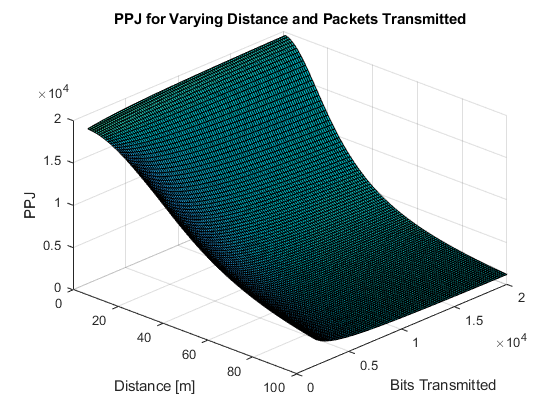
\includegraphics[width=0.45\textwidth]{Images/solutionSpace2ndLayer.png}
  \label{fig:solspace2ndlayer}}
  \hfill
  \subfloat[Solution space for data transmission energy cost for a CH dependent on number of connected child nodes and distance to the sink.]{
  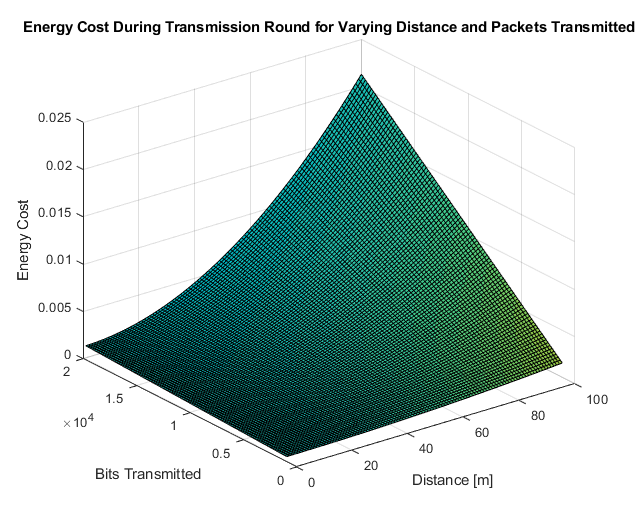
\includegraphics[width=0.45\textwidth]{Images/EnergyCost2ndLayer.png}
  \label{fig:nrjcost2ndLayer}}
  \caption{The solution space for a CH with regards to data transmission energy cost and PPJ.}
  \label{fig:optimizationProbMatlab}
\end{figure}





\subsubsection{Free Nodes}
During almost every clustering period, a number of nodes find themselves closer to the sink than to any nearby CH. These stay connected during the whole transmission round while the sink is moving around. Since these nodes are not being controlled, they were left out of the objective function in order to reduce the computational load further. However, one important observation is that the free nodes under these circumstances are almost always at their closest to their receiver before the sink starts moving. Therefore, all non-CHs were set to send their mandatory package during the first time segment.

\subsubsection*{Practical Method}
The ULC class takes the form of an extension to the environment engine, see Figure \ref{fig:ULCUML}. It works by dynamically building a new model for the current transmission round by polling for which nodes are currently CHs and then stores the state values of the CHs and defines the intermediate equations governing the objectives and constraints. \newline 

\begin{figure}
    \centering
    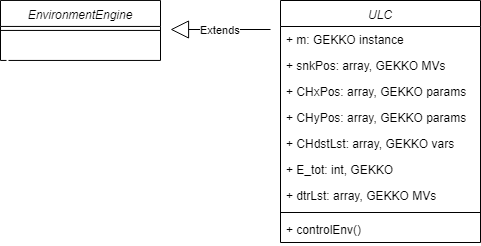
\includegraphics[scale = 0.45]{Images/ULCUML.png}
    \caption{The ULC with its additional functions and attributes as an extension of the Environment Engine class. The GEKKO instance (m) solves for an optimal value for its MVs (each element in dtrLst and snkPos) in order to maximize $bit/J$.}
    \label{fig:ULCUML}
\end{figure}

\noindent The beginning of the implementation process consisted of developing requirements such as:
\begin{itemize}
    \item The optimizer shall produce control inputs that yield an estimated increase of system $bit/J$.
    \item The controller shall posses a fail-safe for any case when the optimizer fails to find a solution.
\end{itemize}

\noindent Initially, the controller was validated and tested for optimizing with respect to a one dimensional distance argument; node positions were simplified to randomized parameter values along $[-50,-49,\hdots,50]$. For each added position, a new GEKKO variable was added for each sink-node distance, $\delta_{CH-sink}$ along with its constraint equation as seen in Equation \ref{eq:deltaCHsink} (two dimensional version). The optimizer was then extended to controlling an additional data transmission rate MV, $dtr$, for each node. Finally, the MV for the position of the sink and the multiple $\delta_{CH-sink}$-variables were split up into their corresponding $x$- and $y$-coordinates. To validate the requirement at each step, the control output of the optimizer and its effect was analyzed and compared with the behaviour of a standard uncontrolled LEACH network. This was done with regards to the summed distance between the sink and all controlled nodes as well as the $bit/J$ ratio.  \newline
 
\noindent A fail-safe was also deployed by implementing a catch for the solver in case it should crash. The catch produces a "safe" control input in the same form as a standard LEACH control system would have. Namely, sink positioned in the middle while each CH is required to send the minimum amount of packages.\newline

\noindent While testing the ULC, every generated sink position was recorded to assess the average distance that the sink would want to travel between clusterings. This was done in order to estimate what sink velocity was needed for average performance. 

(value=33.03 MAY BE PLACED IN RESULTS)

\subsubsection{Product}
Once \verb!controlEnv()! is initialized, the optimizer produces outputs as shown in Figure \ref{fig:ULCoutputs}.

\begin{figure}[h]
  \centering
  \subfloat[ULC sink position output. Blue nodes are CHs and their corresponding numbers are their IDs, green nodes are non-CHs connected to a CH, and yellow nodes are free nodes connected directly connected to the sink.]{
  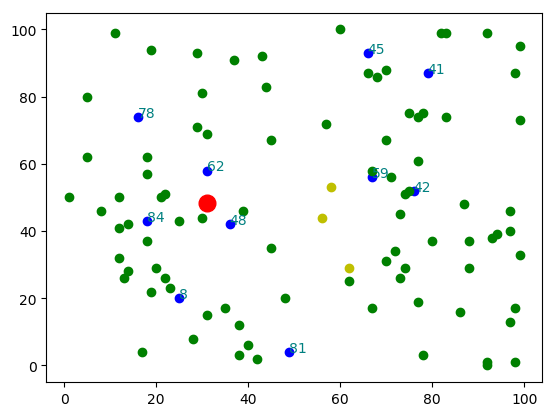
\includegraphics[width=0.45\textwidth]{Images/2ndLayerMap.png}
  \label{fig:ULCmapOutput}}
  \hfill
  \subfloat[ULC $\delta_{d,i}$ output. The desired amount of packages to be sent by each CH with corresponding ID.]{
  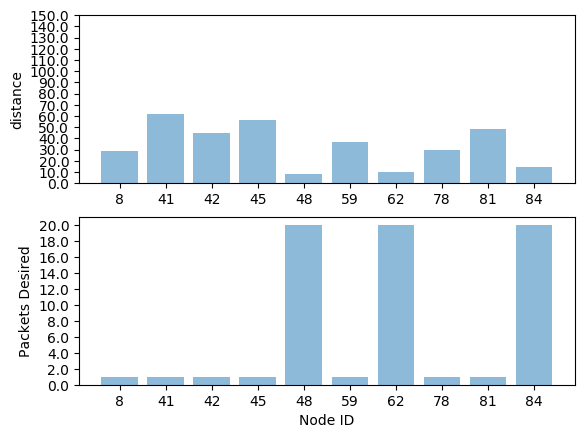
\includegraphics[width=0.45\textwidth]{Images/2ndLayerBar.png}
  \label{fig:ULCbarOutput}}
  \caption{The outputs generated by the ULC. The node ID numbers of a and b are corresponded.}
  \label{fig:ULCoutputs}
\end{figure}


\subsection{Lower Layer Control}
\noindent The LLC aims to optimize for as little energy consumption as possible while still sending the desired amount of packages, $\delta_d$, ordered by the ULC. It does this by controlling the packet rate for each CH during each time segment of the transmission round.\newline  

\noindent The node optimization sub-problem was stated as an objective function consisting of two objectives. Here $\Psi_{node}$ depends on energy consumed by the transmission and $\Phi_{node}$ on the amount of data remaining $\delta_r$ to be sent. The objectives are coupled with weight parameters $Q_{node}$ and $R_{node}$.
\begin{align}
    J_{node}^* = min \: \sum_{n=0}^{K-1} Q\Psi_{node}(k,i,d,b_{tx}) - R\Phi_{node}(K_{deadline},b_{tx}))
\end{align}
Where the objectives were described as
\begin{align}
    \Psi_{node} = E_{Tx}\\
    \Phi{node} = |\delta_r|
\end{align}
The state space model for the node was expressed as
\begin{align}
    E(k+1) = E(k) - (E_{Tx} \\
    \delta_{r}(k+1) = \delta_r(k) - b_{tx}\\
    d(k+1) = v(k)
\end{align}
With state vectors
\begin{align}
    \textbf{x} = [x_{n}, y_{n}, x_{sink}, y_{sink}, \delta_{r}, E]^{T} \\
    \textbf{u} = b_{tx}\\
    \textbf{d} = E_{gen,n}
\end{align}
Subject to constraints for $k\in [0,\hdots,T-1]$
\begin{align}
    0 \leq PA \leq 20 \\
    E \geq [0,\Psi_{node}] \\
\end{align}
The initial states are defined as
\begin{align}
    \delta(0) = \delta_{d}  \\ %delta_desired
    v(0) = v_0
\end{align}

\subsubsection*{Practical Method}
\noindent The following requirements were stated for the LLC:
\begin{itemize}
    \item The optimizer shall produce a control input sequence that result in transmission of as much data as desired by the ULC, or as much as possible if the desired data is an unreachable amount. This data shall be sent before the end of the transmission round.
    \item The controller shall posses a fail-safe for any case when the optimizer fails to find a solution.
\end{itemize}

\noindent The LLC system consists of two cooperating parts, one extension of the Node class and one extension of the Sink class, as shown in Figure \ref{fig:nodeUML}. 

\begin{figure}[h]
  \centering
  \subfloat[Node part of the LLC with  additional functions and attributes as an extension of the Node class. The GEKKO instance (m) solves for an optimal value for its MV (PA during each time segment) in order to minimize the total $\Psi_{node}$.]{
  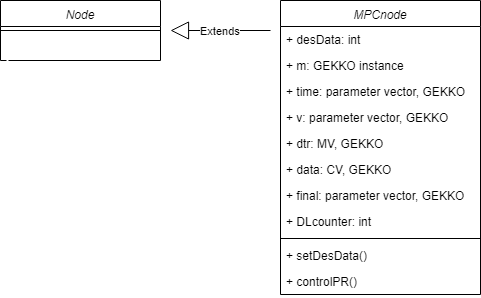
\includegraphics[width=6cm, height=4cm]{Images/nodeUML.png}
  \label{fig:nodeUML}}
  \hfill
  \subfloat[Sink part of the LLC with additional functions and attributes as an extension of the Sink class. MVs are $x$ and $y$ movement.]{
  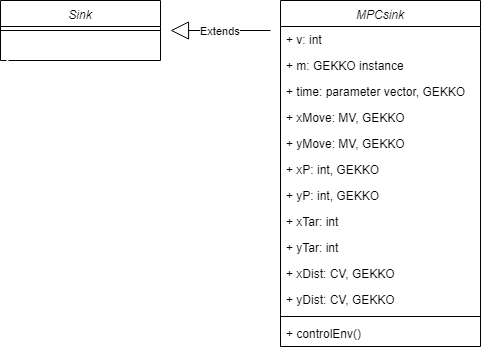
\includegraphics[width=6cm, height=4cm]{Images/sinkUML.png}
  \label{fig:sinkUML}}
  \caption{UML representations of the node and sink extensions.}
  \label{fig:LLCUML}
\end{figure}

\noindent The algorithm starts of by updating the set point of both classes, see Figure \ref{fig:LLCflowchart}. The sink solves for its planned trajectory and stores it in \verb!xP! and \verb!yP!, which can then be polled by any node in order to generate their packet rate control horizon. The trajectory is solved with a fixed horizon length and the endpoint constraint is time-shifted until the current time arrives at the final time constraint ("deadline" in Figure \ref{fig:LLCflowchart}). This is done by coupling the value of $\Psi_{node}$ to a parameter vector \verb!final = [0,...,0,1]! with \verb!length()! equal to the horizon length. The \verb!1! is then shifted as the horizon draws closer to the deadline time constraint. In this case, the final time constraint is always set as the end of the transmission round. A fail-safe was also deployed here with a similar strategy as in the ULC. If no solution is found, the node sends the minimum amount of packages by the end of the transmission round.

\begin{figure}
    \centering
    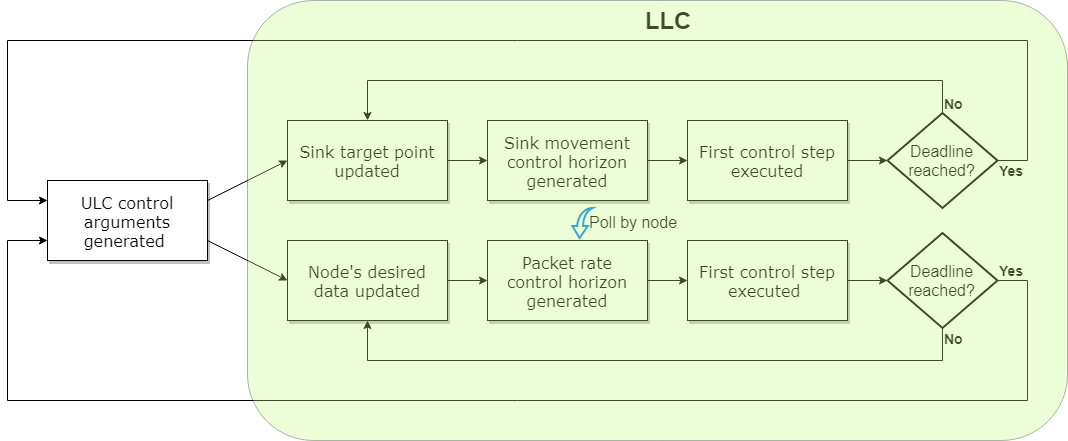
\includegraphics[scale=0.35]{Images/LLCflowchart.png}
    \caption{Flowchart describing the action sequence of the LLC.}
    \label{fig:LLCflowchart}
\end{figure}

\subsubsection{Product}
When \verb!controlPR()! and \verb!produce_MoveVector()! are initialized, the following horizons are generated by the GEKKO modules. See Figure \ref{fig:ULCoutputs}.

\begin{figure}[h]
  \centering
  \subfloat[Control horizon for a node. As shown in the figure, the node plans its transmission for when the sink is at its closest distance (when it passes by).]{
  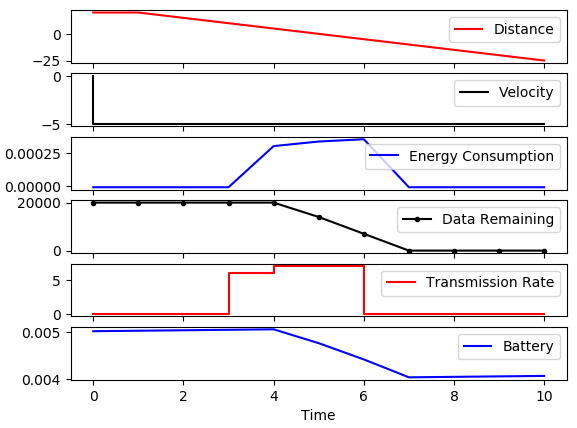
\includegraphics[width=0.45\textwidth]{Images/1stLayerNodePlot.png}
  \label{fig:FirstLayerNode}}
  \hfill
  \subfloat[Control horizon for the sink.]{
  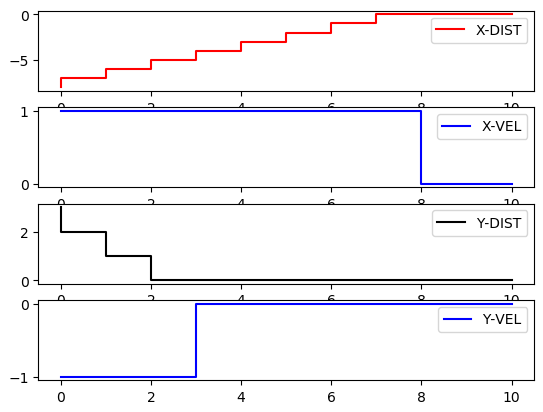
\includegraphics[width=0.45\textwidth]{Images/1stLayerSinkPlot.png}
  \label{fig:FirstLayerSink}}
  \caption{The outputs generated by the LLC. The planned positions of the sink generated by the sink MPC are used by the node MPC in order to plan its transmission timings.}
  \label{fig:LLCoutputs}
\end{figure}

\newpage

\section{RL Design}

\noindent In accordance with the previous discussions on the choice of data driven controller, see Section \ref{sec:ctrlstrategies}, a RL approach was selected. Further, it was decided that the DQN algorithm was the best choice for controlling the mobile sink due to that the WSN environment consisted of a large number of states and actions. The development procedure of the DQN controller was based on the below stated requirements. \newline

\begin{itemize}
    \item The sink/controller shall send as many data packets as possible whilst minimizing the distance to the nodes. 
    \item The amount of states and actions shall be as few as possible to avoid the curse of dimensionality.
    \item The sink shall be movable and the PR of the nodes regulatable.
    \item The controller shall train in the \verb!EnvironmentEngine! simulation environment.
\end{itemize}

\noindent To fulfill the first requirement, the reward was positive for an increase in data packets sent and negative for an increase in distance between the nodes and the sink for the specific case of controlling the sink. The action set $\mathcal{A}$, i.e. the possible actions that the sink could take, was defined as

\begin{equation*}
\begin{multlined}
    \mathcal{A}\:\epsilon\:\{up, down, left, right, diagonal, \\ reduce\:data\:packets\:sent, increase\:data\:packets\:sent\}  
\end{multlined}
\end{equation*}


 \noindent This implies that it was possible for the sink as agent to move right, left, up, down and diagonally with a predetermined step length as well as adjusting the PR of all the nodes. All the states that the agent could be in were determined by a combination of the position of the sink, CH status of all nodes and PR of all nodes. \newline

\noindent Due to the reasoning in Section \ref{sec:softwaretools} regarding the machine learning tools, it was decided to use TensorFlow with Keras running on top of it. The Keras API was deployed to set up the NN and to tune its weights with a built-in optimizer. Based on the mean absolute error of the NN, the optimizer updated the weights such that the loss in Equation \ref{eq:mse} was minimized. Furthermore, the gym library developed by OpenAI was used to setup the WSN in a RL context. \newline

\noindent For controlling the mobile sink with a DQN, the amount of neurons in the input layer of the NN corresponded to the number of states and the amount of neurons in the output layer corresponded to the amount of actions. Thereby the only parameters that needed to be designed were the amount of hidden layers, the amount of neurons in each hidden layer and the learning parameters i.e. the learning rate $\alpha$, discount factor $\gamma$ and the exploration rate $\epsilon$.

% These design choices will be described further in Subsection \ref{sec:RLdesignchoices}.     

\subsection{Design choices}
\label{sec:RLdesignchoices}
In order to design a reliable and fast learned RL controller, several design choices needed to be made. This subsection will declare, describe and motivate the choices that were made during the design of the RL controller.  

\begin{itemize}
    \item \textbf{Learning rate $\alpha$} --- The learning rate shall be in the order of $10^{-3}$, as stated by Thoma \cite{Thoma2017}. If $\alpha$ is too small the learning process will be longer and if $\alpha$ is too large the learning will not converge. Since the time factor is not of priority in this study, the learning rate was chosen to be $10^{-2}$. \newline
    \newline
    \noindent Furthermore, the learning rate was made to adapt to changes in the environment by using a state of the art NN optimizer called Adam-optimizer. A study has found that adapting the learning rate using the Adam-optimizer outperforms a range of other optimizers \cite{kingma2014adam}.

    \item \textbf{Discount factor $\gamma$} --- The discount factor is a variable which determines the amount of future steps the agent will consider when an action is chosen. According to Leissner et al. the discount factor needs to be close to 1 to take actions that are very future oriented \cite{Liessner2019}. The authors also claim that if the discount factor is low the agent will be short sighted and thereby drain its battery immediately. The main challenge was to achieve energy savings at the moment as well as to consider the impacts in the long term. Hence, a decision was made to select the discount factor as $0.8$. 
    
    \item \textbf{Exploration rate $\epsilon$} --- To answer the research question: \textit{"How is the $\epsilon$ value to be selected concerning exploration versus exploitation for the data driven optimal control?"}, both a fix and a decaying exploration rate were implemented twice with varying $\epsilon$-values. The fixed $\epsilon$-values were selected as $0.1$ and $0.15$. The reason for this was that a large $\epsilon$-value would cause the agent to frequently select an deficient action during the late phase of training when it has already built up a relatively good model of the environment. \newline  
    
    \noindent To explore the large number of states and actions of the WSN environment, the initial exploration rate was chosen to be as large as possible for the decaying $\epsilon$ tests, namely $1$. After each action, $\epsilon$ was decayed by multiplying the current exploration rate with a decay factor. The exploration rate was decreased by following the previous procedure until it reached a predefined minimum exploration rate. For the decaying $\epsilon$ tests, the decay factors were set to $0.9995$ \& $0.995$ and the minimum exploration rates were set to $0.05$ \& $0.01$ respectively for the two tests. See Table \ref{tb:epsilonchoice} for a summary of the different exploration rates that were tested. Note that the initial exploration rates were the $\epsilon$-values that were used throughout the entire learning process for the fixed $\epsilon$ tests.
        
    \begin{table}[h!]
        \centering
        \caption{Choices of exploration rate}
        \label{tb:epsilonchoice}
        \begin{tabular}{llcccll}
            \toprule
                     &        &\textbf{Initial $\epsilon$} & \textbf{$\epsilon$ decay factor} & \textbf{$\epsilon$ minimum}\\
            \midrule
         Decaying $\epsilon$  & Test 1 & 1 & 0.9995 & 0.05\\
                     & Test 2 & 1 & 0.995 &  0.01\\ \midrule
         Fix $\epsilon$       & Test 1 & 0.15 & n/a &  n/a\\ 
                     & Test 2 & 0.1 & n/a &  n/a\\
            \bottomrule
        \end{tabular}
    \end{table}

    
    \item \textbf{Reward} --- For the WSN environment a positive reward was given for an increase in amount of data packets sent and a negative reward was given for an increase in distance between the sink and the nodes. The rewards for the two factors were tuned based on multiple trials of various ratios between the two reward factors. Based on constant learning parameters, i.e $\alpha$, $\gamma$ and $\epsilon$ along with the outcome of each trial the rewards were changed such that the desired behaviour was achieved. For instance, if the agent survived a large number of rounds but sent few packets, the reward factor for the amount of data packets sent was increased.
    
    \item \textbf{Amount of hidden layers} --- The accuracy of a NN will increase if the amount of hidden layers are increased until a point when the learning is saturated and the accuracy will start to decrease \cite{he2016deep}. Implementing many hidden layers will also increase the computational load and it is usually enough to use 2 hidden layers according to Heaton \cite{heaton2015artificial}. Due to what was discussed above, 2 hidden layers was chosen for the sink controller. 
    
    \item \textbf{Amount of neurons in hidden layers} --- According to the rule of thumb the amount of neurons in the hidden layers shall be less than double the amount of neurons in the input layer \cite{heaton2015artificial}. The decision was made to select 24 neurons and 48 neurons for the first hidden layer and the second hidden layer respectively.     
\end{itemize}

\noindent Table \ref{tb:RLdesign} below summarizes the choices of the design parameters and Algorithm \ref{alg:dqn} depicts the DQN algorithm in pseudo code. 

\begin{table}[h!]
    \centering
    \caption{RL design parameter choices}
    \label{tb:RLdesign}
    \begin{tabular}{ 
        l % left aligned column
        l % left aligned column
        *{3}{S[table-format=4.0]} % three columns with numeric data       
    }
        \toprule
        \textbf{Parameter} & \textbf{Value}  \\ 
        \midrule
        Learning rate, $\alpha$ & $0.01$ \\
        Discount factor, $\gamma$ & $0.8$ \\
        Optimizer & Adam \\ 
        No. of hidden layers & 2 \\
        No. of neurons in hidden layer 1  & $24$ \\
        No. of neurons in hidden layer 2  & $48$ \\
        \bottomrule
    \end{tabular}
\end{table}


\begin{algorithm}
\caption{DQN Algorithm}\label{alg:dqn}
\begin{algorithmic}[1]
\State Import libraries 
\State Create instance of WSN environment
\State Create and build NN model 
\For{Amount of training episodes}
    \While{At least one node still alive}
        \State Randomize \textit{value} between $0$ and $1$
        \If{\textit{value} <= $\epsilon$}
            \State Select random action 
        \Else 
            \State Predict action with largest Q-value with NN
        \EndIf
        \State Sink in WSN environment implements the action
        \State Observe reward gained \& append info onto memory array
        \State Update weights of NN by randomly sampling from memory array
        \If{\textbf{not} fixed $\epsilon$}
            \State Decay $\epsilon$ by multiplying with the decay rate
        \EndIf{ \textbf{not}}
    \EndWhile
\EndFor
\end{algorithmic}
\end{algorithm}





\begin{comment}
\subsection{Control Method One, Model Based MPC Approach}
\noindent Model predictive control (MPC) is a control method that is based on solving an open loop optimization problem which contains the system model. The controller development was divided into three sequential parts and this subsection will delve deeper into these parts. 

\paragraph{\textit{Defining the Dynamic Features of the Controlled Objective}}
\noindent 
\noindent \newline The equations governing the energy and data aggregation dynamics of each node in the system is derived from \cite{heinzelman2000energy} and are expressed as
\begin{flalign}
    E_{Tz}(k,d) &= E_{elec}k+\epsilon k d^{2} \\
    E_{Rz}(k) &= E_{elec}*k
\end{flalign}
where $k$ is amount of bits, $d$ is the distance between transmitter and receiver, and $E_{Tz}$ and $E_{Rz}$ are energy used for transmission and receiving respective. Here, a CH does both while non-CHs only do transmitting. Each node's $SoC$ is also able to stochastically generate a relatively small amount of energy during each time step. The movement of the sink is simplified by constraining only it's step size, i.e. the movement dynamics themselves are seen as non-existent. 

\paragraph{\textit{Stating the Control Problem}}
\noindent 
\noindent\newline
The progression of the system from one time step to another could be expressed by the discrete state transitions in the form $x(k+1)=f(x(k),u(k))$. The system takes a nonlinear form due to several reasons. One is the probabilistic CH role assignment. Another is the stochastic variation of connected nodes to each CH and the energy generated by each node. One can also observe that the control signal $PA_i$ is coupled with the non-linear state representation $d_i$, which makes the system control affine \cite{PlanningAlgorithms}.\newline

\noindent The states, control inputs, and outputs are described in vector form as respective $x$, $u$, and $y$ are described as follows
\begin{equation}
\label{x_k}
    x =
    \begin{bmatrix}
        x_{sink} \\
        y_{sink} \\
        x_{1,..,N} \\
        y_{1,..,N} \\
        CHS_{1,..,N} \\
        PS_{1,..,N} \\
        EC_{1,..,N} 
    \end{bmatrix}, \:
    u = 
    \begin{bmatrix}
        \Delta x_{sink} \\
        \Delta y_{sink} \\
        \Delta PA_{1,..,N}
    \end{bmatrix}, \:
    y = 
    \begin{bmatrix}
        0 & 0 & 0 & 0 & 0 & 1 & 1
    \end{bmatrix}
\end{equation}
\noindent where $(\Delta x_{sink}, \Delta y_{sink})$ is the change in position of the sink. The position of node $i\in{\{1,...,j\}}$ nodes is assumed to be static. $PS_i$ is the amount of packets sent, $PA_i$ is a control input deciding how many packets to send each control step depending on the distance $d_i$ from each node $i$ to the sink, and $EC_i$ is energy consumed. Here, CH status, $CHS_i \in [0,1]$ is an indicator of whether the node has been chosen to be a CH or not which would decide if control is to be executed with regards to that node. We get a state space representation such that $x(k+1) = Ax + GBu$ and $y=Cx$. However, with an increasing number of nodes the dimension of the state space increases exponentially.
\paragraph{\textit{Choice of Solving Method\newline}}
\hspace{-0.6cm} \noindent To solve the problem of the ever increasing dimensionality, a strategy involving breaking the optimization problem for the entire state-space into minor optimization problems was formed; one for each node and one for the sink. The outputs of these are then summarized in a greater optimization problem which in turn generates the control inputs for the system.
\noindent A cost function $C(x,u)$ dependent on both economic goals was then to be formed with appropriate weighting parameters.

\end{comment}
